\section{Durchführung}
\label{sec:Durchführung}

Bei der Bestimmung der Wärmeleitfähigkeit werden zwar unterschiedliche Methoden 
verwendet, alleridngs bleibt der Aufbau gleich und ist in \autoref{fig:peltier}
zu sehen.
\begin{figure}[h]
    \centering
        \centering
        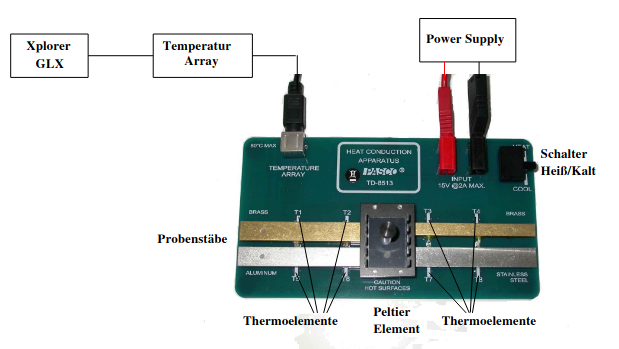
\includegraphics[width=\textwidth]{Bilder/peltier.png}
        \caption{Aufbau zur Bestimmung der Leitfähigkeit. \cite{peltier}}
    \hfill
    \label{fig:peltier}
\end{figure}
Die Metallstreifen links und rechts des Peltier-Elements, bestehen aus Messing
(oberer Streifen), Aluminium (unten links) und Edelstahl (unten rechts). Das 
Peltier-Element ist mit einer Spannungsquelle verbunden und wandelt die 
zugeführte Energie in Wärme um, sodass die Stäbe erhitzt werden. Die Temperatur 
wird mithilfe eines Thermoelements gemessen, welches über ein Temperatur Array 
an einen Datenlogger angeschlossen ist, an dem die Abtastraten noch verändert
wertden (siehe unten). Um Wärmeverluste zu vermeiden wird eine Wärmeisolierung
auf die Stäbe gelegt, dann wird der obere rechte Schalter auf "HEAT" geschaltet, 
sodass die Energie-Wärme-Umwandlung im Peltier-Element beginnt.
Nach jeder Messung werden diese Isolierungen wieder abgenommen und der obere
Schalter auf "COOL" gestellt, sodass die Stäbe langsam wieder abkühlen.

\subsection{Statische Methode}
Hierbei wird zunächst die Abtastrate $\Delta t_{GLX}$ des Datenloggers auf 10s
eingestellt und die Ausgangsspannung der Spannungsquelle auf $U_0$ = 5V 
eingestellt. Der Heizvorgang findet statt bis eine Temperatur von 
45°C erreicht ist. Im späteren Verlauf wird bestimmt, welcher Stab die beste 
Wärmeleitfähigkeit hat, dazu werden die Temperaturen der Thermoelemente T1, T4, T5 und T8 
nach 700s festgehalten und verglichen.

\subsection{Dynamische Methode}
Bei der dynamischen Methode wird das Angström-Messverfahren verwendet, bei der 
der Probenstab periodisch erhitzt wird. Zunächst wird $\Delta t_{GLX}$ von 10 auf 
2s gesetzt. An der Spannungsquelle werden $U_P$ = 8V angelegt. Sobald alle
Stäbe auf 30°C heruntergekühlt, kann die Messung losgehen, diese sieht wie
folgt aus: Für 40s wird geheizt, dann wird 40s gekühlt. Diese 80s Perioden
werden 11 mal wiederholt.
\\
Genau das Gleiche wird jetzt für eine Periodendauer mit 200s wiederholt. Die 
Messung wird beendet, sobald eines der Thermoelemente eine Temperatur von 80°C 
erreicht.